\section{Dark photon model}
\label{sec:model}

\newcommand{\zdgauge}{\ensuremath{\mathrm{U(1)}_D}\xspace}

A detailed description of the dark photon model is given in~\cite{Curtin:2014cca}. This section gives a brief 
introduction to the model. The model is defined by a \zdgauge gauge sector and a SM singlet $S$ with unit charge 
under \zdgauge. The kinematic terms for the dark sector in the lagrangian can be written as 

\begin{equation}
L_{\mathrm{gauge,dark}} = -\frac{1}{4} B_{\mu\nu}B^{\mu\nu} - \frac{1}{4} Z_{\mu\nu}Z^{\mu\nu} + \frac{1}{2} \frac{\epsilon}{\cos \theta_W} Z_{\mu\nu}Z^{\mu\nu}
\end{equation}
where $B$ and $Z$ are vector fields before kinematic mixing and $\theta_W$ is the usual Weinberg angle. In addition, 
the Higgs potential is
\begin{equation}
V_0 = -\mu^2 \left| H \right|^2 + \lambda \left| H \right|^4 -\mu_D^2 \left| S \right|^2 + \lambda \left| S \right|^4 + \kappa \left| H \right|^2 \left| S \right|^2
\end{equation}
where $S$ is the dark Higgs field. Similar to SM, the dark Higgs gives a vacuum expection value and the \zd 
acquires a non-zero mass. Connections between the SM and dark sector depend on the kinematic mixing parameter 
$\epsilon$ and the Higgs mixing $\kappa$. Possible Feynman diagrams with exotic Higgs decays to four leptons are 
shown in Figure~\ref{fig:feyn_zd}. $\epsilon$ controls decay widths of Higgs to a $Z$ boson and \zd and $\kappa$ 
controls that of Higgs to \zd \zd. In this analysis, $\kappa$ is assumed to have a negligible value to suppress 
contributions from the dark Higgs mixing.

\begin{figure}[!htb]
\begin{center}
    {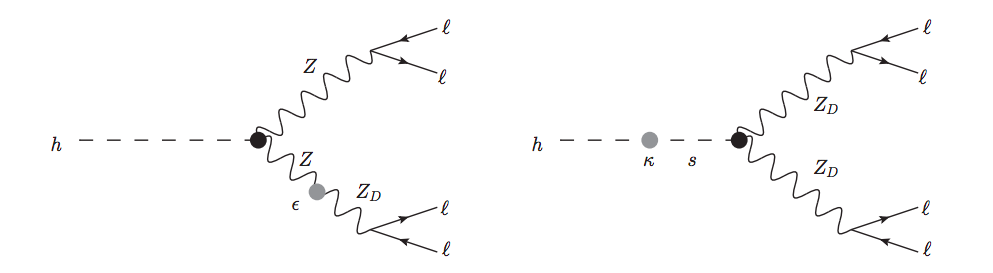
\includegraphics [width=0.75\textwidth] {Figures/Model/zdfeyn}}
\caption{
Exotic Higgs decays to four leptons via intermediate dark photons in the hypercharge portal (left) and Higgs portal (right).
}
\label{fig:feyn_zd}
\end{center}
\end{figure}
